\documentclass[11pt]{article}
\usepackage[margin=1in]{geometry}
\usepackage{amsmath,amssymb,amsthm,mathtools}
\usepackage{graphicx}
\usepackage{booktabs,longtable,array,tabularx}
\usepackage{enumitem}
\usepackage{hyperref}
\usepackage{float}
\usepackage{multirow}
\usepackage{pdflscape}
\usepackage{tikz}
\usetikzlibrary{arrows.meta,positioning,shapes.geometric}

\hypersetup{
  colorlinks=true,
  linkcolor=black,
  urlcolor=blue,
  citecolor=black
}

\title{Decentralized Perishable Inventory Model with Delayed Transshipment and Emergency Orders:\\
Final Report}
\author{}
\date{}

\begin{document}
\maketitle

\begin{abstract}
This report documents the current decentralized perishable inventory model and matches the mathematics to the implemented simulation. The model has two facilities, a three-period inventory life cycle (new, medium, old, then expiry), first-expire-first-out (FEFO) issuing, regular warehouse replenishment with lead times, a one-period transshipment lead from node B to node A, and a one-period emergency warehouse order available to node A. Safety stock is set using a newsvendor-style cost ratio, and continuous review is treated as the default operating baseline while periodic review is retained only as a benchmark reference.

The main purpose of the analysis is to answer two questions within that continuous-review baseline. First, how should the newsvendor-style cost structure be set when underage and overage incentives differ? Second, during a surge at period 7, should A rely on node B transshipment or place an emergency warehouse order? To answer those questions, the report compares two cost regimes: one in which underage cost exceeds overage cost, and one in which overage cost exceeds underage cost. The results show that node B transshipment is the better emergency response in both regimes. In the underage-dominant case, transshipment and emergency ordering produce the same service improvement, but transshipment is materially cheaper. In the overage-dominant case, transshipment remains economical while the emergency order is too expensive to justify at the assumed expedited price.
\end{abstract}

\section{Introduction}
This report studies a decentralized perishable inventory system with two facilities. Facility A is the stressed node in the experiments and facility B is the donor node in the transshipment tests. The model uses three usable inventory ages (new, medium, old), a one-period transshipment lead from B to A, a one-period emergency warehouse order available to A, and continuous review as the default operating baseline.

Those modeling choices matter. Delayed transshipment cannot eliminate same-period shortage; it can only reduce future backlog. Emergency warehouse orders behave the same way in timing terms because they also arrive one period later, but they arrive as new inventory and carry a much higher unit cost. The three-age structure makes inventory age operationally important because medium stock can still be shipped, whereas old stock is too close to expiry to survive the trip. Continuous review is used as the default baseline because the March periodic benchmark is too unstable to serve as the main operating case.

This report therefore has four goals:
\begin{enumerate}[leftmargin=2em]
\item define the updated notation and equations so they match the implemented model;
\item collect the cost setup in one place, including safety stock, response triggers, and total-cost accounting;
\item present the final sensitivity analysis under the continuous-review baseline and under two different cost regimes;
\item interpret the results and provide a recommendation for how the model should be set up going forward.
\end{enumerate}

\section{System Description}
The model represents a two-node decentralized system over a finite planning horizon. Facility A and facility B face stochastic demand, place replenishment orders to a warehouse, and carry perishable inventory. Demand is generated using a fixed random seed so that alternative policies are tested on the same demand path. The horizon contains $T=15$ periods and is grouped into cycles of three periods for reporting convenience.

Figure~\ref{fig:system-flow} summarizes the within-period operating flow used throughout the report.

\begin{figure}[H]
\centering
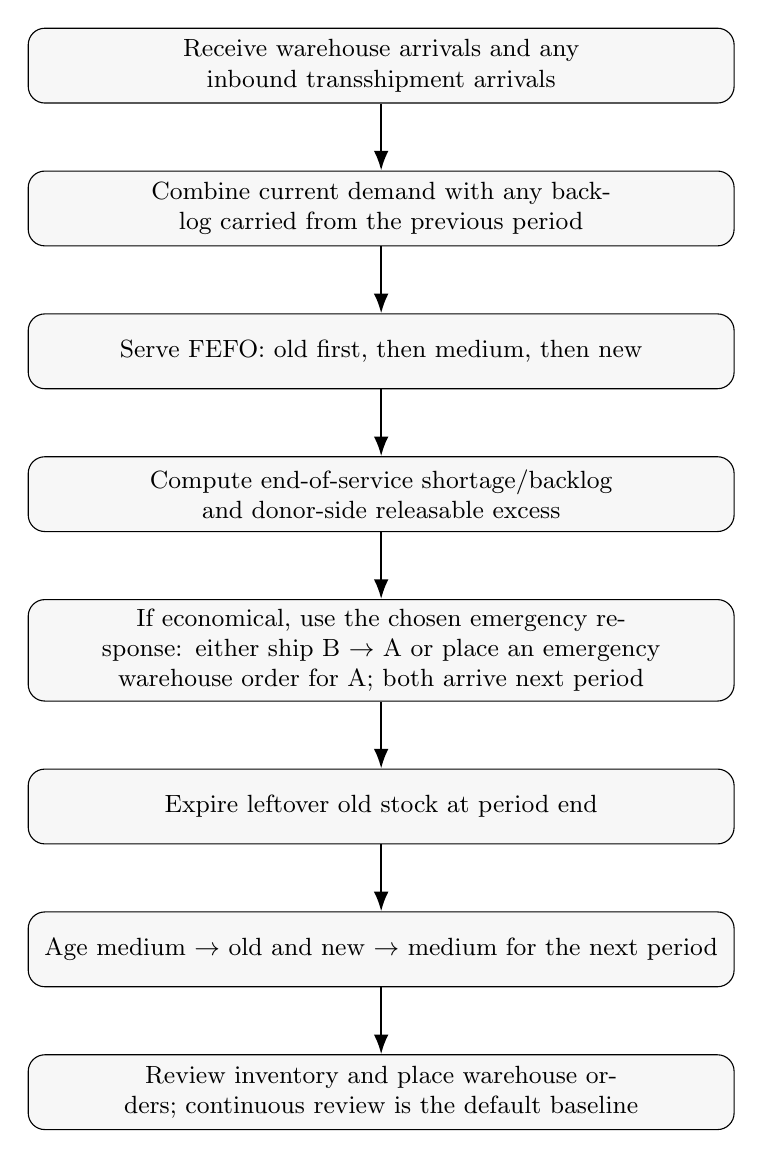
\begin{tikzpicture}[
  node distance=0.85cm,
  every node/.style={font=\small},
  flowstep/.style={
    rectangle,
    rounded corners=6pt,
    draw=black,
    align=center,
    text width=0.72\textwidth,
    minimum width=0.72\textwidth,
    minimum height=0.95cm,
    fill=gray!6
  },
  arrow/.style={-{Latex[length=2.5mm]}, thick}
]
\node[flowstep] (s1) {Receive warehouse arrivals and any inbound transshipment arrivals};
\node[flowstep, below=of s1] (s2) {Combine current demand with any backlog carried from the previous period};
\node[flowstep, below=of s2] (s3) {Serve FEFO: old first, then medium, then new};
\node[flowstep, below=of s3] (s4) {Compute end-of-service shortage/backlog and donor-side releasable excess};
\node[flowstep, below=of s4] (s5) {If economical, use the chosen emergency response: either ship B $\rightarrow$ A or place an emergency warehouse order for A; both arrive next period};
\node[flowstep, below=of s5] (s6) {Expire leftover old stock at period end};
\node[flowstep, below=of s6] (s7) {Age medium $\rightarrow$ old and new $\rightarrow$ medium for the next period};
\node[flowstep, below=of s7] (s8) {Review inventory and place warehouse orders; continuous review is the default baseline};

\draw[arrow] (s1) -- (s2);
\draw[arrow] (s2) -- (s3);
\draw[arrow] (s3) -- (s4);
\draw[arrow] (s4) -- (s5);
\draw[arrow] (s5) -- (s6);
\draw[arrow] (s6) -- (s7);
\draw[arrow] (s7) -- (s8);
\end{tikzpicture}
\caption{Within-period operating flow of the current model.}
\label{fig:system-flow}
\end{figure}

The final analysis uses a no-surge baseline and a separate single-period surge at period 7. The surge multiplies A's demand by $2.0$ while leaving B's demand unchanged. This design allows the baseline to be understood first and then the emergency-response comparison to be evaluated separately.

\section{Sets, Indices, and Notation}
\subsection{Sets and Indices}
\begin{align*}
\mathcal{I} &:= \{A,B\} && \text{set of facilities},\\
\mathcal{T} &:= \{1,2,\dots,T\} && \text{set of periods},\\
\mathcal{G} &:= \{n,m,o\} && \text{inventory ages: new, medium, old}.
\end{align*}

\subsection{Parameters}
\begin{longtable}{>{\raggedright\arraybackslash}p{0.19\linewidth} p{0.76\linewidth}}
\toprule
Parameter & Meaning \\
\midrule
$T$ & total number of periods in the simulation horizon \\
$d_{i,t}$ & realized demand at facility $i$ in period $t$ \\
$\mu_i, \sigma_i$ & mean and standard deviation of demand for facility $i$ \\
$L_i$ & warehouse replenishment lead time for facility $i$ \\
$R_i$ & review cycle length for facility $i$ in the periodic benchmark \\
$r_i$ & reorder point for facility $i$ \\
$S_i$ & order-up-to level for facility $i$ \\
$\delta_{i,t}$ & review indicator, equal to 1 if facility $i$ is allowed to review and order in period $t$ \\
$\lambda_i$ & donor reserve retained before facility $i$ is allowed to transship inventory \\
$ss_i$ & safety stock at facility $i$ derived from the newsvendor cost ratio \\
$K$ & fixed ordering cost per order event \\
$h_i$ & holding cost per end-of-period usable unit at facility $i$ \\
$\phi_i$ & expiry cost per expired unit at facility $i$ \\
$c^{tr}$ & transshipment cost per unit moved from B to A \\
$c^{new}$ & additional surcharge paid by the receiving node per fresh unit received via transshipment \\
$c^{em}$ & emergency warehouse order cost per unit expedited to A \\
$\ell_i$ & lost profit or waiting cost per backlogged unit per period at facility $i$ \\
$\tau$ & usable product lifespan, equal to 3 periods in this report \\
$\hat{w}_{i,t}$ & estimated waiting periods if backlog at facility $i$ is not transshipped in period $t$ \\
$C^{\max}$ & maximum number of units that may be transshipped in one period \\
$I^{n}_{i,0}$ & initial new inventory at facility $i$ at the start of period 1 \\
$\kappa_i$ & continuous-review order-coverage parameter used to set $S_i$ in the continuous policy \\
\bottomrule
\end{longtable}

\subsection{State Variables and Flow Variables}
\begin{longtable}{>{\raggedright\arraybackslash}p{0.19\linewidth} p{0.76\linewidth}}
\toprule
Variable & Meaning \\
\midrule
$I^{n}_{i,t}, I^{m}_{i,t}, I^{o}_{i,t}$ & new, medium, and old inventory available at the start of period $t$ after arrivals \\
$u^{n}_{i,t}, u^{m}_{i,t}, u^{o}_{i,t}$ & units issued locally from new, medium, and old inventory in period $t$ \\
$B_{i,t}$ & end-of-period backlog at facility $i$ \\
$s_{i,t}$ & newly unmet demand in period $t$ at facility $i$ \\
$a_{i,t}$ & warehouse order arrival received by facility $i$ in period $t$ \\
$q_{i,t}$ & warehouse replenishment order placed by facility $i$ in period $t$ \\
$z^{m}_{B,A,t}$ & medium units sent from B to A in period $t$; these arrive at A next period as old units \\
$z^{n}_{B,A,t}$ & new units sent from B to A in period $t$; these arrive at A next period as medium units \\
$y^{em}_{A,t}$ & emergency warehouse units expedited to A in period $t$; these arrive next period as new units \\
$e_{i,t}$ & expired units at facility $i$ in period $t$ \\
$IP_{i,t}$ & inventory position used to trigger an order at the end of period $t$ \\
\bottomrule
\end{longtable}

\section{Cost Setup}
\label{sec:cost-setup}
This section collects the cost logic in one place. The rest of the report uses these definitions instead of reintroducing costs inside each operating rule.

\subsection{Cost Components}
The simulation uses seven cost components:
\begin{itemize}[leftmargin=2em]
\item lost-profit waiting cost, $\ell_i B_{i,t}$, charged for demand still waiting at the end of the period;
\item fixed ordering cost, $K \mathbf{1}_{\{q_{i,t}>0\}}$, charged whenever a facility places a warehouse order;
\item holding cost, $h_i H_{i,t}$, charged for usable inventory carried into the next period;
\item expiry cost, $\phi_i e_{i,t}$, charged when old inventory expires;
\item transshipment cost, charged per unit when B sends inventory to A;
\item fresh-unit receiving surcharge, charged only when B sends new inventory to A;
\item emergency order cost, charged per unit when A uses expedited warehouse replenishment.
\end{itemize}
The shared cost settings that do not change by regime are
\begin{align*}
c^{tr} &= 1.2, &
c^{new} &= 2.0, &
c^{em} &= 6.0, &
K &= 35.
\end{align*}
Here $c^{tr}$ is the transshipment cost per unit, $c^{new}$ is the extra receiver-side surcharge per fresh unit, $c^{em}$ is the expedited emergency warehouse cost per unit, and $K$ is the fixed cost per regular warehouse order event.

\subsection{Cost Regimes}
Two cost structures are tested. These regimes change lost profit, holding, and expiry weights while keeping the shared transshipment and ordering costs above fixed.

\begin{table}[H]
\centering
\caption{Cost regimes used in the sensitivity analysis}
\label{tab:cost-regimes}
\begin{tabular}{lccccc}
\toprule
Regime & $\ell_i$ & $h_A$ & $h_B$ & $\phi_A$ & $\phi_B$ \\
\midrule
Underage $>$ Overage & 12.0 & 0.35 & 0.30 & 2.5 & 2.5 \\
Overage $>$ Underage & 2.0 & 1.00 & 0.95 & 4.0 & 4.0 \\
\bottomrule
\end{tabular}
\end{table}

The underage-dominant case represents an environment in which lost profit from waiting demand is much more costly than carrying or expiring inventory. The overage-dominant case represents a leaner environment in which excess stock is heavily penalized and waiting demand is comparatively more acceptable.

\subsection{Safety Stock and Service Level}
Safety stock is derived from the classical newsvendor logic, but it is used here as a policy input into a simulation rather than as part of a one-shot static decision. The key idea is to map the cost of being short to the cost of carrying too much and then translate that cost ratio into a target service level.

For each facility $i$, define the protection period
\begin{align}
P_i =
\begin{cases}
R_i + L_i, & \text{periodic review},\\
L_i, & \text{continuous review}.
\end{cases}
\end{align}

The underage cost is
\begin{align}
Cu_i = \ell_i P_i,
\end{align}
which treats underage as lost profit per unit per period across the protection period. There is no separate immediate shortage penalty. The overage proxy is
\begin{align}
Co_i = \tau h_i + \phi_i, \qquad \tau=3.
\end{align}
The factor $\tau=3$ appears because the product has a three-period usable life. This overage term is still a proxy rather than a literal claim that every extra unit will be held for exactly three periods and then expire. It is used to set a conservative service target by balancing the pressure to avoid lost profit against the pressure to avoid excess inventory.

The raw newsvendor service level is
\begin{align}
\alpha_i^{raw} = \frac{Cu_i}{Cu_i + Co_i}.
\end{align}
In the current implementation, that service level is capped below by 0.50 and above by 0.999:
\begin{align}
\alpha_i = \min\{\max(\alpha_i^{raw},0.50),0.999\}.
\end{align}
The lower cap prevents negative or implausibly lean safety stock values when overage dominates underage. The corresponding standard-normal value is
\begin{align}
z_i = \Phi^{-1}(\alpha_i),
\end{align}
and safety stock is then
\begin{align}
ss_i = \left\lceil z_i \sigma_i \sqrt{P_i} \right\rceil.
\end{align}

The values $Cu_i$ and $Co_i$ are not the full operating cost function by themselves. They determine a service target that feeds the ordering and donor-retention rules. The full simulation cost is still composed of lost-profit waiting, transshipment, emergency ordering, regular ordering, holding, and expiry costs.

\subsection{Emergency Response Cost Triggers}
The model estimates how long A would wait if no emergency response occurs. In practice, this is the wait until the next useful replenishment arrival, usually a warehouse order already in the pipeline or a new warehouse order after lead time. That estimated waiting time is denoted $\hat{w}_{A,t}$, and the receiver-side penalty signal becomes
\begin{align}
\rho_{A,t} = \ell_A \hat{w}_{A,t}.
\end{align}
This is not a comparison against the fixed cost of placing a warehouse order. It is a comparison between \emph{responding now} and \emph{letting A wait for replenishment}. Base transshipment is allowed only if
\begin{align}
c^{tr} < \rho_{A,t},
\end{align}
and fresh-unit transshipment is allowed only if
\begin{align}
c^{tr} + c^{new} < \rho_{A,t}.
\end{align}
Emergency ordering is allowed only if
\begin{align}
c^{em} < \rho_{A,t}.
\end{align}
Here $c^{new}$ is interpreted as a receiver-side surcharge: if A asks for fresh stock from B, A pays an extra fee for receiving that fresher inventory. The physical limits on how much B can send are described later in the transshipment mechanics. The emergency order has no donor-side inventory limit, but it is allowed only in the emergency-order response scenario and only for node A.

\subsection{Evaluation Objective and Accounting}
The simulator reports the realized total cost
\begin{align}
\text{TC} =
\sum_{t \in \mathcal{T}} \sum_{i \in \mathcal{I}}
\left(
\ell_i B_{i,t}
+ K \mathbf{1}_{\{q_{i,t}>0\}}
+ h_i H_{i,t}
+ \phi_i e_{i,t}
\right)
+ \sum_{t \in \mathcal{T}} \left(c^{tr} z^m_{B,A,t} + (c^{tr}+c^{new}) z^n_{B,A,t} + c^{em} y^{em}_{A,t}\right),
\end{align}
where $H_{i,t}=I^o_{i,t+1}+I^m_{i,t+1}$ is end-of-period usable on-hand inventory. In the tables, the term
\begin{align}
\ell_i B_{i,t}
\end{align}
is reported as \emph{lost-profit cost}. Shortage is still tracked operationally, but the cost accounting now charges only the period-by-period cost of demand that remains backlogged.

At the node level, the model assigns the base shipping cost $c^{tr}$ to the shipping node, the fresh-unit surcharge $c^{new}$ to the receiving node, and the emergency warehouse charge $c^{em} y^{em}_{A,t}$ to node A. That accounting rule does not change system total cost, but it does change how node A and node B costs are interpreted in the detailed tables.

\section{Methodology}
\subsection{Demand Process}
For each facility and period, demand is drawn from a normal distribution and rounded to the nearest nonnegative integer:
\begin{align}
d_{i,t} = \max\{0,\text{round}(\mathcal{N}(\mu_i,\sigma_i^2))\}.
\end{align}
The random seed is fixed at 42 so that every policy is evaluated on the same demand path. In the surge experiment, demand at A in period 7 is multiplied by 2.0, while B's demand is left unchanged.

\subsection{Inventory Aging and FEFO Service}
Warehouse arrivals enter the system as new inventory, and emergency warehouse arrivals enter the system as new inventory as well:
\begin{align}
a_{i,t} =
\begin{cases}
q_{i,t-L_i}, & t-L_i \ge 1,\\
0, & \text{otherwise},
\end{cases}
\end{align}
and
\begin{align}
I^n_{i,t} = a_{i,t} + a^{em}_{i,t} + \mathbf{1}_{\{t=1\}} I^n_{i,0},
\end{align}
where $a^{em}_{i,t}=0$ for $i=B$ and, for A,
\begin{align}
a^{em}_{A,t} =
\begin{cases}
y^{em}_{A,t-1}, & t \ge 2,\\
0, & t=1.
\end{cases}
\end{align}

At the start of period $t$, backlog from the previous period is combined with current demand:
\begin{align}
\tilde{d}_{i,t} = d_{i,t} + B_{i,t-1},
\end{align}
with $B_{i,0}=0$. The system then serves first-expire-first-out (FEFO), which means old inventory is used before medium inventory, and medium inventory is used before new inventory:
\begin{align}
u^o_{i,t} &= \min\{I^o_{i,t}, \tilde{d}_{i,t}\},\\
u^m_{i,t} &= \min\{I^m_{i,t}, \tilde{d}_{i,t} - u^o_{i,t}\},\\
u^n_{i,t} &= \min\{I^n_{i,t}, \tilde{d}_{i,t} - u^o_{i,t} - u^m_{i,t}\}.
\end{align}
Total local service is
\begin{align}
U_{i,t} = u^o_{i,t} + u^m_{i,t} + u^n_{i,t}.
\end{align}

Because backlog is served ahead of current demand, newly unmet demand is defined separately from end backlog. The backlog satisfied in period $t$ is
\begin{align}
v_{i,t} = \min\{B_{i,t-1}, U_{i,t}\},
\end{align}
so service devoted to current-period demand is
\begin{align}
U^{cur}_{i,t} = U_{i,t} - v_{i,t}.
\end{align}
Newly unmet demand is therefore
\begin{align}
s_{i,t} = \max\{0, d_{i,t} - U^{cur}_{i,t}\},
\end{align}
while end backlog is
\begin{align}
B_{i,t} = \max\{0, B_{i,t-1} + d_{i,t} - U_{i,t}\}.
\end{align}

\subsection{Delayed Transshipment Mechanics}
After local service, the donor can only transship medium or new stock. Leftover old stock cannot survive the trip because transshipment takes one full period and old inventory would expire before it becomes useful to the receiver. Let post-service leftovers at B be
\begin{align}
L^o_{B,t} = I^o_{B,t} - u^o_{B,t}, \quad
L^m_{B,t} = I^m_{B,t} - u^m_{B,t}, \quad
L^n_{B,t} = I^n_{B,t} - u^n_{B,t}.
\end{align}

The donor's releasable excess is
\begin{align}
g_{B,t} = \max\{0, L^m_{B,t} + L^n_{B,t} - \lambda_B - ss_B\}.
\end{align}
This rule means B must retain its transshipment reserve and its safety stock before it is allowed to help A.

The cost test in Section~\ref{sec:cost-setup} determines whether medium and new units are economical to send. If $B_{A,t}^{pre}$ denotes A's backlog immediately after local service but before any new shipment is sent, then the transshipment quantities are
\begin{align}
z^m_{B,A,t} &= \min\{B_{A,t}^{pre}, L^m_{B,t}, g_{B,t}, C^{\max}\},\\
z^n_{B,A,t} &= \min\{B_{A,t}^{pre} - z^m_{B,A,t}, L^n_{B,t}, g_{B,t} - z^m_{B,A,t}, C^{\max} - z^m_{B,A,t}\},
\end{align}
with $z^n_{B,A,t}=0$ whenever fresh-unit transshipment is not economical.

The one-period transshipment lead has a specific aging implication:
\begin{align}
\text{medium shipped at } t &\rightarrow \text{arrives at A in } t+1 \text{ as old},\\
\text{new shipped at } t &\rightarrow \text{arrives at A in } t+1 \text{ as medium}.
\end{align}

\subsection{Emergency Warehouse Order Mechanics}
The emergency warehouse order is an alternative response used only in the emergency-order scenario. It is available only to node A. If $B_{A,t}^{pre}$ denotes A's backlog immediately after local service but before any emergency response, then the expedited order quantity is
\begin{align}
y^{em}_{A,t} =
\begin{cases}
B_{A,t}^{pre}, & \text{if } c^{em}<\rho_{A,t},\\
0, & \text{otherwise}.
\end{cases}
\end{align}
The order is placed at the end of period $t$, arrives in period $t+1$, and arrives as new inventory. Because the emergency lead time is still one period, the expedited order cannot eliminate same-period shortage. It can only reduce next-period backlog, exactly like delayed transshipment.

\subsection{Aging, Expiry, and State Transition}
After local service and any outbound transshipment, leftover old inventory expires:
\begin{align}
e_{i,t} = L^o_{i,t}.
\end{align}
The remaining medium stock ages into old, and the remaining new stock ages into medium:
\begin{align}
I^o_{i,t+1} &= \left(L^m_{i,t} - z^m_{i,\cdot,t}\right) + \sum_{j \ne i} z^m_{j,i,t},\\
I^m_{i,t+1} &= \left(L^n_{i,t} - z^n_{i,\cdot,t}\right) + \sum_{j \ne i} z^n_{j,i,t}.
\end{align}
In the current final experiments, only B is allowed to send to A, so the only nonzero transshipment terms are $z^m_{B,A,t}$ and $z^n_{B,A,t}$.

\subsection{Ordering Rules}
The model uses an order-up-to policy in both review modes, but the trigger mechanism differs.

\paragraph{Periodic benchmark.}
Facility $i$ reviews only when $\delta_{i,t}=1$, where
\begin{align}
\delta_{i,t} =
\begin{cases}
1, & t \equiv 0 \pmod{R_i},\\
0, & \text{otherwise}.
\end{cases}
\end{align}
Inventory position at the end of the period is
\begin{align}
IP_{i,t} = I^o_{i,t+1} + I^m_{i,t+1} + \text{on-order}_{i,t} + \text{inbound transshipment}_{i,t} + \text{inbound emergency}_{i,t} - B_{i,t}.
\end{align}
On review periods, the order is
\begin{align}
q_{i,t} = \max\left\{0,\left(S_i + ss_i\right) - IP_{i,t}\right\}
\quad \text{if } IP_{i,t} \le r_i + ss_i.
\end{align}

\paragraph{Continuous review sensitivity.}
Continuous review checks inventory every period, so $\delta_{i,t}=1$ for all $t$. In that case, the protection period shrinks from $R_i+L_i$ to $L_i$, and the continuous policy uses pre-configured reorder points and order-up-to levels:
\begin{align}
r_i^{cont} &= \left\lceil \mu_i L_i + ss_i \right\rceil,\\
S_i^{cont} &= \left\lceil \mu_i (L_i + \kappa_i) + ss_i \right\rceil.
\end{align}
The corresponding order rule is
\begin{align}
q_{i,t} = \max\left\{0, S_i^{cont} - IP_{i,t}\right\}
\quad \text{if } IP_{i,t} \le r_i^{cont}.
\end{align}

This continuous policy is not meant to represent a perfect global optimum. It is a structured sensitivity test whose purpose is to create a smoother baseline so that transshipment can be interpreted as an emergency mechanism rather than as a substitute for weak replenishment timing.

\section{Experimental Design}
\subsection{Shared Structural Settings}
Table~\ref{tab:shared-structure} reports the structural parameters shared across the final experiments.

\begin{table}[H]
\centering
\caption{Shared structural settings}
\label{tab:shared-structure}
\begin{tabular}{lll}
\toprule
Item & Facility A & Facility B \\
\midrule
Demand mean $\mu_i$ & 43 & 35 \\
Demand standard deviation $\sigma_i$ & 4 & 3 \\
Periodic review cycle $R_i$ & 4 & 3 \\
Lead time $L_i$ & 2 & 3 \\
Periodic reorder point $r_i$ & 95 & 80 \\
Periodic order-up-to $S_i$ & 140 & 210 \\
Initial on-hand inventory & 100 & 210 \\
Reserve for transshipment $\lambda_i$ & 35 & 35 \\
\bottomrule
\end{tabular}
\end{table}

Additional shared assumptions are:
\begin{itemize}[leftmargin=2em]
\item planning horizon $T=15$ periods;
\item three-period product life: new $\rightarrow$ medium $\rightarrow$ old $\rightarrow$ expiry;
\item transshipment lead time of 1 period;
\item emergency warehouse order lead time of 1 period, with arrival as new inventory;
\item transshipment direction B $\rightarrow$ A only in the sensitivity study;
\item transshipment cap $C^{\max}=70$ units per period;
\item emergency warehouse unit cost $c^{em}=6.0$ for node A;
\item random seed 42;
\item one-period surge at period 7 with multiplier 2.0 on A only.
\end{itemize}

\subsection{Continuous-Review Configuration}
The continuous-review setup changes three tuning choices relative to the periodic benchmark:
\begin{align*}
\kappa_A &= 0.4, &
\kappa_B &= 1.8, &
\lambda_B^{cont} &= 5.
\end{align*}
These values are easier to read in plain language:
\begin{itemize}[leftmargin=2em]
\item $\kappa_A=0.4$ means A orders to cover its lead time plus about 0.4 extra periods of demand. This keeps A relatively lean, so the surge can still create stress.
\item $\kappa_B=1.8$ means B orders to cover its lead time plus about 1.8 extra periods of demand. This gives B more buffer so it can act as a donor when A is hit by the surge.
\item $\lambda_B^{cont}=5$ means that in the continuous-review experiment, B must keep only 5 extra units before sharing, in addition to its safety stock. In the periodic benchmark the reserve was much higher, so B was more protected and less able to help.
\end{itemize}
So the continuous-review test is intentionally designed to make A the stressed node and B the emergency backup node. A is kept lean enough that the surge still matters, while B is given enough coverage and a lower reserve so that transshipment can actually happen.

\section{Results}
\subsection{Safety Stock and Service Levels}
Using the cost setup in Section~\ref{sec:cost-setup}, Table~\ref{tab:ss-metrics} reports the exact newsvendor metrics used in the final runs.

\begin{table}[H]
\centering
\caption{Safety stock metrics by regime and review mode}
\label{tab:ss-metrics}
\begin{tabular}{llccccccc}
\toprule
Regime & Mode & Facility & $P_i$ & $Cu_i$ & $Co_i$ & $\alpha_i$ & $z_i$ & $ss_i$ \\
\midrule
\multirow{4}{*}{Underage $>$ Overage}
& Periodic & A & 6 & 72.00 & 3.55 & 0.953 & 1.675 & 17 \\
& Periodic & B & 6 & 72.00 & 3.40 & 0.955 & 1.694 & 13 \\
& Continuous & A & 2 & 24.00 & 3.55 & 0.871 & 1.132 & 7 \\
& Continuous & B & 3 & 36.00 & 3.40 & 0.914 & 1.364 & 8 \\
\midrule
\multirow{4}{*}{Overage $>$ Underage}
& Periodic & A & 6 & 12.00 & 7.00 & 0.632 & 0.336 & 4 \\
& Periodic & B & 6 & 12.00 & 6.85 & 0.637 & 0.349 & 3 \\
& Continuous & A & 2 & 4.00 & 7.00 & 0.500$^{a}$ & 0.000 & 0 \\
& Continuous & B & 3 & 6.00 & 6.85 & 0.500$^{a}$ & 0.000 & 0 \\
\bottomrule
\end{tabular}
\begin{flushleft}
\footnotesize $^{a}$The raw $\alpha_i$ values are below 0.50 in the continuous overage-dominant case. The implementation floors them at 0.50 to avoid negative or nonsensical safety-stock targets.
\end{flushleft}
\end{table}

The table has the same qualitative message as before. Continuous review shortens the protection period and therefore reduces safety stock relative to the periodic benchmark. Underage-dominant costs create positive safety stock under both review modes. Overage-dominant costs push the continuous-review service target to the floor and collapse safety stock to zero. That difference matters later because it changes how exposed A is before the surge and how much releasable stock B has available to help.

\subsection{Benchmark Reference for the Continuous Baseline}
Table~\ref{tab:baseline-comparison} compares the no-surge baseline under the March periodic benchmark and under the continuous-review baseline used in this report.

\begin{table}[H]
\centering
\caption{Baseline comparison with no imposed surge}
\label{tab:baseline-comparison}
\small
\begin{tabularx}{\textwidth}{@{}l *{6}{>{\centering\arraybackslash}X}@{}}
\toprule
Regime & \shortstack{Periodic\\shortage} & \shortstack{Periodic\\cum. backlog} & \shortstack{Periodic\\total cost} & \shortstack{Continuous\\shortage} & \shortstack{Continuous\\cum. backlog} & \shortstack{Continuous\\total cost} \\
\midrule
Underage $>$ Overage & 444 & 716 & 9663 & 34 & 34 & 1792 \\
Overage $>$ Underage & 470 & 768 & 3420 & 34 & 34 & 2104 \\
\bottomrule
\end{tabularx}
\end{table}

Continuous review remains the right baseline. In both regimes, it cuts total shortage from more than 440 units to 34 units. The periodic benchmark is too unstable to serve as the main emergency-response case because too much of the transshipment or emergency-order benefit would just be compensating for weak replenishment timing.

\begin{table}[H]
\centering
\caption{Continuous-review no-surge baseline breakdown by node}
\label{tab:continuous-baseline-node-breakdown}
\begin{tabular}{lrrrr}
\toprule
Regime & A shortage & B shortage & A total cost & B total cost \\
\midrule
Underage $>$ Overage & 0 & 34 & 662 & 1129 \\
Overage $>$ Underage & 0 & 34 & 812 & 1292 \\
\bottomrule
\end{tabular}
\end{table}

The remaining baseline shortage still comes entirely from B. A is fully protected before the surge in both regimes. The 34-unit shortage is B's early stockout before its next regular warehouse arrival. This matters because the surge experiment is meant to test how A should respond once it becomes stressed, not whether B's own baseline pipeline is perfect.

\subsection{Surge Response Under Continuous Review}
The final question is no longer ``transship or do nothing.'' It is whether A should rely on node B or use an emergency warehouse order once the period-7 surge creates backlog. Table~\ref{tab:surge-summary} compares the three response scenarios.

\begin{table}[H]
\centering
\caption{Surge-at-period-7 results under continuous review}
\label{tab:surge-summary}
\small
\setlength{\tabcolsep}{4pt}
\resizebox{\textwidth}{!}{%
\begin{tabular}{llrrrrrrrr}
\toprule
Regime & Response & \shortstack{Shortage\\A+B} & \shortstack{Cum. backlog\\A+B} & \shortstack{Units\\transshipped} & \shortstack{Emergency\\units} & \shortstack{Lost-profit\\cost} & \shortstack{Transship\\cost} & \shortstack{Emergency\\cost} & \shortstack{Total\\cost} \\
\midrule
Underage $>$ Overage & Warehouse only & 76 & 76 & 0 & 0 & 912 & 0.00 & 0.00 & 2280 \\
Underage $>$ Overage & Use node B & 56 & 56 & 22 & 0 & 672 & 26.40 & 0.00 & 2047 \\
Underage $>$ Overage & Emergency order & 56 & 56 & 0 & 22 & 672 & 0.00 & 132.00 & 2173 \\
\midrule
Overage $>$ Underage & Warehouse only & 90 & 90 & 0 & 0 & 180 & 0.00 & 0.00 & 2186 \\
Overage $>$ Underage & Use node B & 68 & 68 & 22 & 0 & 136 & 26.40 & 0.00 & 2105 \\
Overage $>$ Underage & Emergency order & 90 & 90 & 0 & 0 & 180 & 0.00 & 0.00 & 2186 \\
\bottomrule
\end{tabular}
}
\end{table}

Underage-dominant costs create the clearest tradeoff. Both active responses reduce shortage from 76 to 56 and reduce lost-profit cost from 912 to 672. The service improvement is the same because both responses deliver 22 useful units to A in period 8. The difference is price. Node B transshipment costs only 26.40, whereas the emergency order costs 132.00. That is why total cost falls to 2047 under transshipment but only to 2173 under emergency ordering. In the underage-dominant regime, transshipment is better than emergency ordering by about 125.

Overage-dominant costs create a different result. Transshipment still reduces shortage from 90 to 68 and total cost from 2186 to 2105, because the 22 medium units from B remain economical. The emergency order does nothing. Its cost per unit is 6.0, while A's period-7 waiting signal is only 2.0, so the expedited order is not economical and the emergency-order scenario collapses to the same result as warehouse only.

\begin{table}[H]
\centering
\caption{Shortage breakdown in the continuous-review surge runs}
\label{tab:shortage-breakdown}
\begin{tabular}{llrrr}
\toprule
Regime & Response & A shortage & B shortage & Total shortage \\
\midrule
Underage $>$ Overage & Warehouse only & 42 & 34 & 76 \\
Underage $>$ Overage & Use node B & 22 & 34 & 56 \\
Underage $>$ Overage & Emergency order & 22 & 34 & 56 \\
Overage $>$ Underage & Warehouse only & 56 & 34 & 90 \\
Overage $>$ Underage & Use node B & 34 & 34 & 68 \\
Overage $>$ Underage & Emergency order & 56 & 34 & 90 \\
\bottomrule
\end{tabular}
\end{table}

Table~\ref{tab:shortage-breakdown} shows that the response effect is still concentrated at A. B's shortage stays at 34 in all six runs because it is the same early baseline stockout. The response decision changes only A. Underage-dominant transshipment and emergency ordering both reduce A shortage from 42 to 22. Overage-dominant transshipment reduces A shortage from 56 to 34, while emergency ordering leaves A unchanged because no emergency order is placed.

\begin{table}[H]
\centering
\caption{Economic response audit at period 7}
\label{tab:response-audit}
\small
\begin{tabularx}{\textwidth}{@{}lrrrr>{\raggedright\arraybackslash}X>{\raggedright\arraybackslash}X@{}}
\toprule
Regime & $\rho_{A,7}$ & Medium cost & Fresh cost & Emergency cost & Transshipment response & Emergency-order response \\
\midrule
Underage $>$ Overage & 12.0 & 1.2 & 3.2 & 6.0 & Send 22 medium units & Place 22 emergency units \\
Overage $>$ Underage & 2.0 & 1.2 & 3.2 & 6.0 & Send 22 medium units & No order; emergency is too expensive \\
\bottomrule
\end{tabularx}
\end{table}

This table explains why the policies split. In the underage-dominant case, A's one-period waiting signal is 12.0, so medium transshipment, fresh transshipment, and emergency ordering are all economical. Even then, the actual transshipment is only 22 medium units because that is all B can release after protecting its own reserve and safety stock. In the overage-dominant case, the waiting signal is only 2.0. Medium transshipment at 1.2 is still worth doing, but fresh transshipment at 3.2 and emergency ordering at 6.0 are both too expensive. That is why the emergency-order scenario places no order at all in that regime.

\begin{table}[H]
\centering
\caption{Cost improvement relative to warehouse-only response}
\label{tab:response-delta}
\begin{tabular}{llrr}
\toprule
Regime & Response & Shortage improvement & Cost improvement \\
\midrule
Underage $>$ Overage & Use node B & 20 & 233 \\
Underage $>$ Overage & Emergency order & 20 & 107 \\
Overage $>$ Underage & Use node B & 22 & 80 \\
Overage $>$ Underage & Emergency order & 0 & 0 \\
\bottomrule
\end{tabular}
\end{table}

Table~\ref{tab:response-delta} is the cleanest decision table in the report. In the underage-dominant case, transshipment and emergency ordering achieve the same service gain, but transshipment delivers more than twice the economic benefit. In the overage-dominant case, transshipment is the only active response because the emergency order is priced out by the lower waiting penalty.

\subsection{What Happens Around the Surge}
Tables~\ref{tab:underage-focus} and~\ref{tab:overage-focus} isolate periods 6 through 9 so that the timing of the response can be read directly.

\begin{table}[H]
\centering
\caption{Period 6--9 focus: underage-dominant regime}
\label{tab:underage-focus}
\small
\setlength{\tabcolsep}{4pt}
\resizebox{\textwidth}{!}{%
\begin{tabular}{llrrrrrrr}
\toprule
Response & Period & Demand A & Shortage A & End backlog A & B $\rightarrow$ A medium & Emergency units & Order A & Total cost \\
\midrule
Warehouse only & 6 & 47 & 0 & 0 & 0 & 0 & 47 & 64 \\
Warehouse only & 7 & 86 & 22 & 22 & 0 & 0 & 86 & 345 \\
Warehouse only & 8 & 45 & 20 & 20 & 0 & 0 & 45 & 302 \\
Warehouse only & 9 & 44 & 0 & 0 & 0 & 0 & 44 & 88 \\
\midrule
Use node B & 6 & 47 & 0 & 0 & 0 & 0 & 47 & 64 \\
Use node B & 7 & 86 & 22 & 22 & 22 & 0 & 64 & 364 \\
Use node B & 8 & 45 & 0 & 0 & 0 & 0 & 45 & 50 \\
Use node B & 9 & 44 & 0 & 0 & 0 & 0 & 44 & 82 \\
\midrule
Emergency order & 6 & 47 & 0 & 0 & 0 & 0 & 47 & 64 \\
Emergency order & 7 & 86 & 22 & 22 & 0 & 22 & 64 & 477 \\
Emergency order & 8 & 45 & 0 & 0 & 0 & 0 & 45 & 63 \\
Emergency order & 9 & 44 & 0 & 0 & 0 & 0 & 44 & 88 \\
\bottomrule
\end{tabular}
}
\end{table}

\begin{table}[H]
\centering
\caption{Period 6--9 focus: overage-dominant regime}
\label{tab:overage-focus}
\small
\setlength{\tabcolsep}{4pt}
\resizebox{\textwidth}{!}{%
\begin{tabular}{llrrrrrrr}
\toprule
Response & Period & Demand A & Shortage A & End backlog A & B $\rightarrow$ A medium & Emergency units & Order A & Total cost \\
\midrule
Warehouse only & 6 & 47 & 0 & 0 & 0 & 0 & 47 & 111 \\
Warehouse only & 7 & 86 & 29 & 29 & 0 & 0 & 86 & 154 \\
Warehouse only & 8 & 45 & 27 & 27 & 0 & 0 & 45 & 147 \\
Warehouse only & 9 & 44 & 0 & 0 & 0 & 0 & 44 & 113 \\
\midrule
Use node B & 6 & 47 & 0 & 0 & 0 & 0 & 47 & 111 \\
Use node B & 7 & 86 & 29 & 29 & 22 & 0 & 64 & 159 \\
Use node B & 8 & 45 & 5 & 5 & 0 & 0 & 45 & 82 \\
Use node B & 9 & 44 & 0 & 0 & 0 & 0 & 44 & 92 \\
\midrule
Emergency order & 6 & 47 & 0 & 0 & 0 & 0 & 47 & 111 \\
Emergency order & 7 & 86 & 29 & 29 & 0 & 0 & 86 & 154 \\
Emergency order & 8 & 45 & 27 & 27 & 0 & 0 & 45 & 147 \\
Emergency order & 9 & 44 & 0 & 0 & 0 & 0 & 44 & 113 \\
\bottomrule
\end{tabular}
}
\end{table}

These tables show the timing clearly. In both regimes, period 7 still ends with backlog because neither transshipment nor emergency ordering arrives instantly. The response effect appears in period 8. Under underage-dominant costs, both transshipment and emergency ordering eliminate A's period-8 shortage, but transshipment does so much more cheaply. Under overage-dominant costs, transshipment reduces period-8 shortage from 27 to 5, while emergency ordering makes no change because the policy does not place the expensive order.

\section{Analysis and Interpretation}
\subsection{Why Continuous Review is Still the Default Baseline}
The periodic benchmark still generates excessive shortage even when no surge is imposed. Under both cost regimes, the no-surge baseline produces more than 440 units of shortage and more than 700 units of cumulative backlog. That is not a clean platform for comparing transshipment to emergency ordering. Continuous review fixes that problem without changing the core structure of the model. The system still has perishability, warehouse lead times, and delayed emergency responses, but it starts from a far more stable state.

\subsection{Transshipment Versus Emergency Ordering}
The final report's main result is that transshipment is the preferred emergency response whenever B has releasable stock. In the underage-dominant regime, transshipment and emergency ordering deliver the same service benefit because both place 22 useful units into A's period-8 inventory. But transshipment pays only 26.40 to do that, while emergency ordering pays 132.00. In other words, emergency ordering buys the same recovery at a much higher price.

The overage-dominant regime gives an even cleaner answer. There, transshipment remains economical because the medium-unit shipping cost of 1.2 is below A's one-period waiting signal of 2.0. The emergency order does not trigger because its cost of 6.0 is too high. So the emergency policy collapses to the warehouse-only result, while transshipment still improves both service and total cost.

\subsection{Why the Period-8 Effect Matters}
Both emergency responses share the same timing limitation: they arrive one period later. That is why period 7 still shows backlog under every active response. The correct interpretation is not that the response failed. The correct interpretation is that the response changes the \emph{recovery path}. This is why the period-8 rows in Tables~\ref{tab:underage-focus} and~\ref{tab:overage-focus} matter more than the period-7 rows when comparing alternatives.

\section{Recommendation}
The strongest recommendation from this analysis is to keep continuous review as the baseline policy for future stress tests. Once that stable baseline is in place, the preferred emergency response is to use node B first whenever B has releasable stock and the transshipment cost remains below A's waiting signal.

The emergency warehouse order should be treated as a fallback, not as the default first response. In the current simulation it is useful only in the underage-dominant regime, and even there it is dominated by transshipment because it achieves the same shortage reduction at a much higher cost. Under the overage-dominant regime it is not economical at all at the assumed expedited price.

Operationally, the most defensible policy story is:
\begin{enumerate}[leftmargin=2em]
\item run the network under continuous review so the normal state is stable;
\item use node B as the first emergency source when A experiences a surge;
\item reserve expedited emergency warehouse orders for cases where B cannot cover the surge and the waiting signal is high enough to justify the premium;
\item keep the one-period response lead in the model so the analysis respects realistic timing rather than assuming same-period rescue.
\end{enumerate}

The main remaining modeling task is calibration. The current analysis is structurally informative, but parameters such as lost profit per unit per period, holding cost, expiry cost, transshipment cost, and emergency order cost still need to be tied to real operational data if the model is to be used for policy recommendation beyond demonstration and sensitivity testing.

\section{Conclusion}
This final report presents the current decentralized perishable inventory model with three usable ages, one-period transshipment lead, FEFO service, cost-based safety stock, continuous-review baseline testing, and an explicit comparison between node B transshipment and emergency warehouse ordering. The analysis shows that continuous review is the appropriate baseline for studying emergency response. Once that baseline is in place, node B transshipment is the preferred response in both tested cost regimes.

The practical implication is straightforward. If the goal is to build a robust model in which emergency actions are reserved for genuine disruptions rather than routine instability, then the system should be analyzed under continuous review and should treat transshipment as the first emergency option whenever donor stock is available. Expedited emergency warehouse orders remain useful as a fallback concept, but at the assumed cost they are dominated by transshipment in the underage-dominant case and are not economical in the overage-dominant case.

\clearpage
\appendix
\section{Period-by-Period Audit Tables}
This appendix adds the detailed period-by-period audit tables requested for interpretation. To keep the appendix readable, the tables below focus on the \emph{transshipment-enabled surge run} under each cost regime, because transshipment is the preferred active response whenever an emergency response is used in the main results. Each regime includes a full node A table, a full node B table, and a full system cost table for that transshipment case. In the cost tables, \emph{node A total cost} includes A's lost-profit waiting cost, any fresh-unit receipt surcharge, order, holding, and expiry costs; \emph{node B total cost} includes B's lost-profit waiting cost, the base shipping cost for outbound transshipment, order, holding, and expiry costs; and the \emph{system total} is the sum of the two node totals.

\begin{landscape}
\scriptsize
\setlength\LTleft{0pt}
\setlength\LTright{0pt}

\subsection{Underage-Dominant Regime: Surge Run with Node B Transshipment}

\begin{longtable}{rrrrrrrrrrrrrr}
\caption{Node A period-by-period state, underage-dominant regime, surge run with transshipment}\label{tab:appendix-underage-a}\\
\toprule
$t$ & Demand & Start BL & Arr old & Arr med & Start old & Start med & Start new & B$\rightarrow$A sent & Short & End BL & Expired & End OH & Order \\
\midrule
\endfirsthead
\toprule
$t$ & Demand & Start BL & Arr old & Arr med & Start old & Start med & Start new & B$\rightarrow$A sent & Short & End BL & Expired & End OH & Order \\
\midrule
\endhead
1 & 44 & 0 & 0 & 0 & 0 & 0 & 111 & 0 & 0 & 0 & 0 & 67 & 44 \\
2 & 46 & 0 & 0 & 0 & 0 & 67 & 0 & 0 & 0 & 0 & 0 & 21 & 46 \\
3 & 35 & 0 & 0 & 0 & 21 & 0 & 44 & 0 & 0 & 0 & 0 & 30 & 35 \\
4 & 44 & 0 & 0 & 0 & 0 & 30 & 46 & 0 & 0 & 0 & 0 & 32 & 44 \\
5 & 43 & 0 & 0 & 0 & 0 & 32 & 35 & 0 & 0 & 0 & 0 & 24 & 43 \\
6 & 47 & 0 & 0 & 0 & 0 & 24 & 44 & 0 & 0 & 0 & 0 & 21 & 47 \\
7 & 86 & 0 & 0 & 0 & 0 & 21 & 43 & 22 & 22 & 22 & 0 & 0 & 64 \\
8 & 45 & 22 & 22 & 0 & 22 & 0 & 47 & 0 & 0 & 0 & 0 & 2 & 45 \\
9 & 44 & 0 & 0 & 0 & 0 & 2 & 64 & 0 & 0 & 0 & 0 & 22 & 44 \\
10 & 47 & 0 & 0 & 0 & 0 & 22 & 45 & 0 & 0 & 0 & 0 & 20 & 47 \\
11 & 42 & 0 & 0 & 0 & 0 & 20 & 44 & 0 & 0 & 0 & 0 & 22 & 42 \\
12 & 48 & 0 & 0 & 0 & 0 & 22 & 47 & 0 & 0 & 0 & 0 & 21 & 48 \\
13 & 41 & 0 & 0 & 0 & 0 & 21 & 42 & 0 & 0 & 0 & 0 & 22 & 41 \\
14 & 45 & 0 & 0 & 0 & 0 & 22 & 48 & 0 & 0 & 0 & 0 & 25 & 45 \\
15 & 45 & 0 & 0 & 0 & 0 & 25 & 41 & 0 & 0 & 0 & 0 & 21 & 45 \\
\bottomrule
\end{longtable}

\begin{longtable}{rrrrrrrrrrrrr}
\caption{Node B period-by-period state, underage-dominant regime, surge run with transshipment}\label{tab:appendix-underage-b}\\
\toprule
$t$ & Demand & Start BL & Start old & Start med & Start new & B$\rightarrow$A med & B$\rightarrow$A new & Short & End BL & Expired & End OH & Order \\
\midrule
\endfirsthead
\toprule
$t$ & Demand & Start BL & Start old & Start med & Start new & B$\rightarrow$A med & B$\rightarrow$A new & Short & End BL & Expired & End OH & Order \\
\midrule
\endhead
1 & 32 & 0 & 0 & 0 & 176 & 0 & 0 & 0 & 0 & 0 & 144 & 0 \\
2 & 38 & 0 & 0 & 144 & 0 & 0 & 0 & 0 & 0 & 0 & 106 & 70 \\
3 & 31 & 0 & 106 & 0 & 0 & 0 & 0 & 0 & 0 & 75 & 0 & 106 \\
4 & 34 & 0 & 0 & 0 & 0 & 0 & 0 & 34 & 34 & 0 & 0 & 0 \\
5 & 32 & 34 & 0 & 0 & 70 & 0 & 0 & 0 & 0 & 0 & 4 & 66 \\
6 & 37 & 0 & 0 & 4 & 106 & 0 & 0 & 0 & 0 & 0 & 73 & 0 \\
7 & 38 & 0 & 0 & 73 & 0 & 22 & 0 & 0 & 0 & 0 & 13 & 97 \\
8 & 32 & 0 & 13 & 0 & 66 & 0 & 0 & 0 & 0 & 0 & 47 & 0 \\
9 & 32 & 0 & 0 & 47 & 0 & 0 & 0 & 0 & 0 & 0 & 15 & 64 \\
10 & 35 & 0 & 15 & 0 & 97 & 0 & 0 & 0 & 0 & 0 & 77 & 0 \\
11 & 33 & 0 & 0 & 77 & 0 & 0 & 0 & 0 & 0 & 0 & 44 & 68 \\
12 & 35 & 0 & 44 & 0 & 64 & 0 & 0 & 0 & 0 & 9 & 64 & 0 \\
13 & 34 & 0 & 0 & 64 & 0 & 0 & 0 & 0 & 0 & 0 & 30 & 78 \\
14 & 36 & 0 & 30 & 0 & 68 & 0 & 0 & 0 & 0 & 0 & 62 & 0 \\
15 & 36 & 0 & 0 & 62 & 0 & 0 & 0 & 0 & 0 & 0 & 26 & 72 \\
\bottomrule
\end{longtable}

\begin{longtable}{rrrrrrrrrrrrrr}
\caption{System cost by period, underage-dominant regime, surge run with transshipment}\label{tab:appendix-underage-cost}\\
\toprule
$t$ & LP cost A & LP cost B & Base ship & Recv surcharge & Order A & Order B & Hold A & Hold B & Exp A & Exp B & Node A total & Node B total & System total \\
\midrule
\endfirsthead
\toprule
$t$ & LP cost A & LP cost B & Base ship & Recv surcharge & Order A & Order B & Hold A & Hold B & Exp A & Exp B & Node A total & Node B total & System total \\
\midrule
\endhead
1 & 0.00 & 0.00 & 0.00 & 0.00 & 35.00 & 0.00 & 23.45 & 43.20 & 0.00 & 0.00 & 58.45 & 43.20 & 101.65 \\
2 & 0.00 & 0.00 & 0.00 & 0.00 & 35.00 & 35.00 & 7.35 & 31.80 & 0.00 & 0.00 & 42.35 & 66.80 & 109.15 \\
3 & 0.00 & 0.00 & 0.00 & 0.00 & 35.00 & 35.00 & 10.50 & 0.00 & 0.00 & 187.50 & 45.50 & 222.50 & 268.00 \\
4 & 0.00 & 408.00 & 0.00 & 0.00 & 35.00 & 0.00 & 11.20 & 0.00 & 0.00 & 0.00 & 46.20 & 408.00 & 454.20 \\
5 & 0.00 & 0.00 & 0.00 & 0.00 & 35.00 & 35.00 & 8.40 & 1.20 & 0.00 & 0.00 & 43.40 & 36.20 & 79.60 \\
6 & 0.00 & 0.00 & 0.00 & 0.00 & 35.00 & 0.00 & 7.35 & 21.90 & 0.00 & 0.00 & 42.35 & 21.90 & 64.25 \\
7 & 264.00 & 0.00 & 26.40 & 0.00 & 35.00 & 35.00 & 0.00 & 3.90 & 0.00 & 0.00 & 299.00 & 65.30 & 364.30 \\
8 & 0.00 & 0.00 & 0.00 & 0.00 & 35.00 & 0.00 & 0.70 & 14.10 & 0.00 & 0.00 & 35.70 & 14.10 & 49.80 \\
9 & 0.00 & 0.00 & 0.00 & 0.00 & 35.00 & 35.00 & 7.70 & 4.50 & 0.00 & 0.00 & 42.70 & 39.50 & 82.20 \\
10 & 0.00 & 0.00 & 0.00 & 0.00 & 35.00 & 0.00 & 7.00 & 23.10 & 0.00 & 0.00 & 42.00 & 23.10 & 65.10 \\
11 & 0.00 & 0.00 & 0.00 & 0.00 & 35.00 & 35.00 & 7.70 & 13.20 & 0.00 & 0.00 & 42.70 & 48.20 & 90.90 \\
12 & 0.00 & 0.00 & 0.00 & 0.00 & 35.00 & 0.00 & 7.35 & 19.20 & 0.00 & 22.50 & 42.35 & 41.70 & 84.05 \\
13 & 0.00 & 0.00 & 0.00 & 0.00 & 35.00 & 35.00 & 7.70 & 9.00 & 0.00 & 0.00 & 42.70 & 44.00 & 86.70 \\
14 & 0.00 & 0.00 & 0.00 & 0.00 & 35.00 & 0.00 & 8.75 & 18.60 & 0.00 & 0.00 & 43.75 & 18.60 & 62.35 \\
15 & 0.00 & 0.00 & 0.00 & 0.00 & 35.00 & 35.00 & 7.35 & 7.80 & 0.00 & 0.00 & 42.35 & 42.80 & 85.15 \\
\bottomrule
\end{longtable}

\subsection{Overage-Dominant Regime: Surge Run with Node B Transshipment}

\begin{longtable}{rrrrrrrrrrrrrr}
\caption{Node A period-by-period state, overage-dominant regime, surge run with transshipment}\label{tab:appendix-overage-a}\\
\toprule
$t$ & Demand & Start BL & Arr old & Arr med & Start old & Start med & Start new & B$\rightarrow$A sent & Short & End BL & Expired & End OH & Order \\
\midrule
\endfirsthead
\toprule
$t$ & Demand & Start BL & Arr old & Arr med & Start old & Start med & Start new & B$\rightarrow$A sent & Short & End BL & Expired & End OH & Order \\
\midrule
\endhead
1 & 44 & 0 & 0 & 0 & 0 & 0 & 104 & 0 & 0 & 0 & 0 & 60 & 44 \\
2 & 46 & 0 & 0 & 0 & 0 & 60 & 0 & 0 & 0 & 0 & 0 & 14 & 46 \\
3 & 35 & 0 & 0 & 0 & 14 & 0 & 44 & 0 & 0 & 0 & 0 & 23 & 35 \\
4 & 44 & 0 & 0 & 0 & 0 & 23 & 46 & 0 & 0 & 0 & 0 & 25 & 44 \\
5 & 43 & 0 & 0 & 0 & 0 & 25 & 35 & 0 & 0 & 0 & 0 & 17 & 43 \\
6 & 47 & 0 & 0 & 0 & 0 & 17 & 44 & 0 & 0 & 0 & 0 & 14 & 47 \\
7 & 86 & 0 & 0 & 0 & 0 & 14 & 43 & 22 & 29 & 29 & 0 & 0 & 64 \\
8 & 45 & 29 & 22 & 0 & 22 & 0 & 47 & 0 & 5 & 5 & 0 & 0 & 45 \\
9 & 44 & 5 & 0 & 0 & 0 & 0 & 64 & 0 & 0 & 0 & 0 & 15 & 44 \\
10 & 47 & 0 & 0 & 0 & 0 & 15 & 45 & 0 & 0 & 0 & 0 & 13 & 47 \\
11 & 42 & 0 & 0 & 0 & 0 & 13 & 44 & 0 & 0 & 0 & 0 & 15 & 42 \\
12 & 48 & 0 & 0 & 0 & 0 & 15 & 47 & 0 & 0 & 0 & 0 & 14 & 48 \\
13 & 41 & 0 & 0 & 0 & 0 & 14 & 42 & 0 & 0 & 0 & 0 & 15 & 41 \\
14 & 45 & 0 & 0 & 0 & 0 & 15 & 48 & 0 & 0 & 0 & 0 & 18 & 45 \\
15 & 45 & 0 & 0 & 0 & 0 & 18 & 41 & 0 & 0 & 0 & 0 & 14 & 45 \\
\bottomrule
\end{longtable}

\begin{longtable}{rrrrrrrrrrrrr}
\caption{Node B period-by-period state, overage-dominant regime, surge run with transshipment}\label{tab:appendix-overage-b}\\
\toprule
$t$ & Demand & Start BL & Start old & Start med & Start new & B$\rightarrow$A med & B$\rightarrow$A new & Short & End BL & Expired & End OH & Order \\
\midrule
\endfirsthead
\toprule
$t$ & Demand & Start BL & Start old & Start med & Start new & B$\rightarrow$A med & B$\rightarrow$A new & Short & End BL & Expired & End OH & Order \\
\midrule
\endhead
1 & 32 & 0 & 0 & 0 & 168 & 0 & 0 & 0 & 0 & 0 & 136 & 0 \\
2 & 38 & 0 & 0 & 136 & 0 & 0 & 0 & 0 & 0 & 0 & 98 & 70 \\
3 & 31 & 0 & 98 & 0 & 0 & 0 & 0 & 0 & 0 & 67 & 0 & 98 \\
4 & 34 & 0 & 0 & 0 & 0 & 0 & 0 & 34 & 34 & 0 & 0 & 0 \\
5 & 32 & 34 & 0 & 0 & 70 & 0 & 0 & 0 & 0 & 0 & 4 & 66 \\
6 & 37 & 0 & 0 & 4 & 98 & 0 & 0 & 0 & 0 & 0 & 65 & 0 \\
7 & 38 & 0 & 0 & 65 & 0 & 22 & 0 & 0 & 0 & 0 & 5 & 97 \\
8 & 32 & 0 & 5 & 0 & 66 & 0 & 0 & 0 & 0 & 0 & 39 & 0 \\
9 & 32 & 0 & 0 & 39 & 0 & 0 & 0 & 0 & 0 & 0 & 7 & 64 \\
10 & 35 & 0 & 7 & 0 & 97 & 0 & 0 & 0 & 0 & 0 & 69 & 0 \\
11 & 33 & 0 & 0 & 69 & 0 & 0 & 0 & 0 & 0 & 0 & 36 & 68 \\
12 & 35 & 0 & 36 & 0 & 64 & 0 & 0 & 0 & 0 & 1 & 64 & 0 \\
13 & 34 & 0 & 0 & 64 & 0 & 0 & 0 & 0 & 0 & 0 & 30 & 70 \\
14 & 36 & 0 & 30 & 0 & 68 & 0 & 0 & 0 & 0 & 0 & 62 & 0 \\
15 & 36 & 0 & 0 & 62 & 0 & 0 & 0 & 0 & 0 & 0 & 26 & 72 \\
\bottomrule
\end{longtable}

\begin{longtable}{rrrrrrrrrrrrrr}
\caption{System cost by period, overage-dominant regime, surge run with transshipment}\label{tab:appendix-overage-cost}\\
\toprule
$t$ & LP cost A & LP cost B & Base ship & Recv surcharge & Order A & Order B & Hold A & Hold B & Exp A & Exp B & Node A total & Node B total & System total \\
\midrule
\endfirsthead
\toprule
$t$ & LP cost A & LP cost B & Base ship & Recv surcharge & Order A & Order B & Hold A & Hold B & Exp A & Exp B & Node A total & Node B total & System total \\
\midrule
\endhead
1 & 0.00 & 0.00 & 0.00 & 0.00 & 35.00 & 0.00 & 60.00 & 129.20 & 0.00 & 0.00 & 95.00 & 129.20 & 224.20 \\
2 & 0.00 & 0.00 & 0.00 & 0.00 & 35.00 & 35.00 & 14.00 & 93.10 & 0.00 & 0.00 & 49.00 & 128.10 & 177.10 \\
3 & 0.00 & 0.00 & 0.00 & 0.00 & 35.00 & 35.00 & 23.00 & 0.00 & 0.00 & 268.00 & 58.00 & 303.00 & 361.00 \\
4 & 0.00 & 68.00 & 0.00 & 0.00 & 35.00 & 0.00 & 25.00 & 0.00 & 0.00 & 0.00 & 60.00 & 68.00 & 128.00 \\
5 & 0.00 & 0.00 & 0.00 & 0.00 & 35.00 & 35.00 & 17.00 & 3.80 & 0.00 & 0.00 & 52.00 & 38.80 & 90.80 \\
6 & 0.00 & 0.00 & 0.00 & 0.00 & 35.00 & 0.00 & 14.00 & 61.75 & 0.00 & 0.00 & 49.00 & 61.75 & 110.75 \\
7 & 58.00 & 0.00 & 26.40 & 0.00 & 35.00 & 35.00 & 0.00 & 4.75 & 0.00 & 0.00 & 93.00 & 66.15 & 159.15 \\
8 & 10.00 & 0.00 & 0.00 & 0.00 & 35.00 & 0.00 & 0.00 & 37.05 & 0.00 & 0.00 & 45.00 & 37.05 & 82.05 \\
9 & 0.00 & 0.00 & 0.00 & 0.00 & 35.00 & 35.00 & 15.00 & 6.65 & 0.00 & 0.00 & 50.00 & 41.65 & 91.65 \\
10 & 0.00 & 0.00 & 0.00 & 0.00 & 35.00 & 0.00 & 13.00 & 65.55 & 0.00 & 0.00 & 48.00 & 65.55 & 113.55 \\
11 & 0.00 & 0.00 & 0.00 & 0.00 & 35.00 & 35.00 & 15.00 & 34.20 & 0.00 & 0.00 & 50.00 & 69.20 & 119.20 \\
12 & 0.00 & 0.00 & 0.00 & 0.00 & 35.00 & 0.00 & 14.00 & 60.80 & 0.00 & 4.00 & 49.00 & 64.80 & 113.80 \\
13 & 0.00 & 0.00 & 0.00 & 0.00 & 35.00 & 35.00 & 15.00 & 28.50 & 0.00 & 0.00 & 50.00 & 63.50 & 113.50 \\
14 & 0.00 & 0.00 & 0.00 & 0.00 & 35.00 & 0.00 & 18.00 & 58.90 & 0.00 & 0.00 & 53.00 & 58.90 & 111.90 \\
15 & 0.00 & 0.00 & 0.00 & 0.00 & 35.00 & 35.00 & 14.00 & 24.70 & 0.00 & 0.00 & 49.00 & 59.70 & 108.70 \\
\bottomrule
\end{longtable}

\subsection{Direct Regime Comparison Around the Surge}
\begin{longtable}{rrrrrrrrrr}
\caption{Periods 6--9 node and system totals laid out side by side}\label{tab:appendix-regime-delta}\\
\toprule
$t$ & U/O Node A & O/U Node A & U/O Node B & O/U Node B & U/O System & O/U System & $\Delta$ A & $\Delta$ B & $\Delta$ System \\
\midrule
\endfirsthead
\toprule
$t$ & U/O Node A & O/U Node A & U/O Node B & O/U Node B & U/O System & O/U System & $\Delta$ A & $\Delta$ B & $\Delta$ System \\
\midrule
\endhead
6 & 42.35 & 49.00 & 21.90 & 61.75 & 64.25 & 110.75 & -6.65 & -39.85 & -46.50 \\
7 & 299.00 & 93.00 & 65.30 & 66.15 & 364.30 & 159.15 & 206.00 & -0.85 & 205.15 \\
8 & 35.70 & 45.00 & 14.10 & 37.05 & 49.80 & 82.05 & -9.30 & -22.95 & -32.25 \\
9 & 42.70 & 50.00 & 39.50 & 41.65 & 82.20 & 91.65 & -7.30 & -2.15 & -9.45 \\
\bottomrule
\end{longtable}

In Table~\ref{tab:appendix-regime-delta}, ``U/O'' denotes the underage-dominant regime and ``O/U'' denotes the overage-dominant regime. The delta columns are computed as \emph{underage-dominant minus overage-dominant}. The surge period itself (period 7) is where the two regimes diverge most sharply at node A, because the higher lost-profit rate in the underage-dominant case makes the same operational event much more expensive at the receiving node. By period 8, both regimes benefit from the 22 units shipped from B, but the underage-dominant case shows the stronger service-based payoff because it completely clears A's backlog.

\end{landscape}

\end{document}
